%%%%%%%%%%%%%%%%%%%%%%%%%%%%%%%%%%%%%%%%%%%%%%%%%%%%%%%%%%%%%%%%%%%%
%% I, the copyright holder of this work, release this work into the
%% public domain. This applies worldwide. In some countries this may
%% not be legally possible; if so: I grant anyone the right to use
%% this work for any purpose, without any conditions, unless such
%% conditions are required by law.
%%%%%%%%%%%%%%%%%%%%%%%%%%%%%%%%%%%%%%%%%%%%%%%%%%%%%%%%%%%%%%%%%%%%

\documentclass[9pt]{beamer}
\usetheme[faculty=fi]{fibeamer}
\usepackage[utf8]{inputenc}
\usepackage[
  main=english, %% By using `czech` or `slovak` as the main locale
                %% instead of `english`, you can typeset the
                %% presentation in either Czech or Slovak,
                %% respectively.
  % czech, slovak %% The additional keys allow foreign texts to be
]{babel}        %% typeset as follows:
%%
%%   \begin{otherlanguage}{czech}   ... \end{otherlanguage}
%%   \begin{otherlanguage}{slovak}  ... \end{otherlanguage}
%%
%% These macros specify information about the presentation
\title{Neutrino Flavor Conversions in Dense Medium: Matter Stimulation, Dispersion Relation, and Neutrino Halo} %% that will be typeset on the
\subtitle{PhD Defense\\ Supervisor: Huaiyu Duan} %% title page.
\author{Lei Ma}

%% These additional packages are used within the document:
\usepackage{ragged2e}  % `\justifying` text
\usepackage{booktabs}  % Tables
\usepackage{tabularx}
\usepackage{tikz}      % Diagrams
\usetikzlibrary{calc, shapes, backgrounds}
\usepackage{amsmath, amssymb}
\usepackage{url}       % `\url`s
\usepackage{listings}  % Code listings

% \usepackage{appendixnumberbeamer}


\usepackage[T1]{fontenc}
% \usefonttheme[onlymath]{serif}
\renewcommand\sfdefault{cmbr}



%\usepackage{booktabs}
%\usepackage[scale=2]{ccicons}
\usepackage{tcolorbox}

%\usepackage{floatrow}

%\usepackage{minted}
%\usemintedstyle{trac}

% For the 68 colors
\usepackage{xcolor}
\definecolor{ao}{rgb}{0.0, 0.5, 0.0}

% \usepackage{pgfplots}
% \usepgfplotslibrary{dateplot}

% \usepackage{xspace}
% \newcommand{\themename}{\textbf{\textsc{metropolis}}\xspace}


\usepackage{subfig}
\usepackage[absolute
,overlay
]{textpos}

%%%%% eso-pic package that set up a grid system for the slides BEGIN
%\usepackage[texcoord,grid,gridcolor=red!10,subgridcolor=green!10,gridunit=pt]{eso-pic}
% grid,gridcolor=red!20,subgridcolor=green!20,gridunit=pt
%%%%% eso-pic package that set up a grid system for the slides END

\usepackage{tikz}



\usepackage{times}
\usepackage{verbatim}
\usetikzlibrary{arrows,shapes}


\usepackage{mathtools}

\newcommand{\verteq}{\rotatebox{90}{$\,=$}}
\newcommand{\equalto}[2]{\underset{\scriptstyle\overset{\mkern4mu\huge \verteq}{#2}}{#1}}


\newcommand{\bra}[1]{\left\langle #1\right|}
\newcommand{\ket}[1]{\left| #1\right\rangle}
\newcommand{\braket}[2]{\langle #1 | #2 \rangle}
\newcommand{\avg}[1]{\left< #1 \right>}
\newcommand{\ii}{\mathrm{i}}
\DeclareMathOperator{\sech}{sech}



\frenchspacing
\begin{document}
  \frame{\maketitle}

%%%%%%%%%%%%%%%%%%%%%%%%%%%%%%%%%%%%%%%%%%%%%%
%%%%%%%%%%%%%%%%
  \AtBeginSection[]{% Print an outline at the beginning of sections
    \begin{frame}<beamer>
      \frametitle{Outline for Section \thesection}
      \tableofcontents[currentsection]
    \end{frame}}

%%%%%%%%%%% Dark Frames
  \begin{darkframes}


    \section{Neutrino Oscillations}

    \subsection{What are Neutrinos}

    \begin{frame}{What are Neutrinos?}

    \begin{figure}
    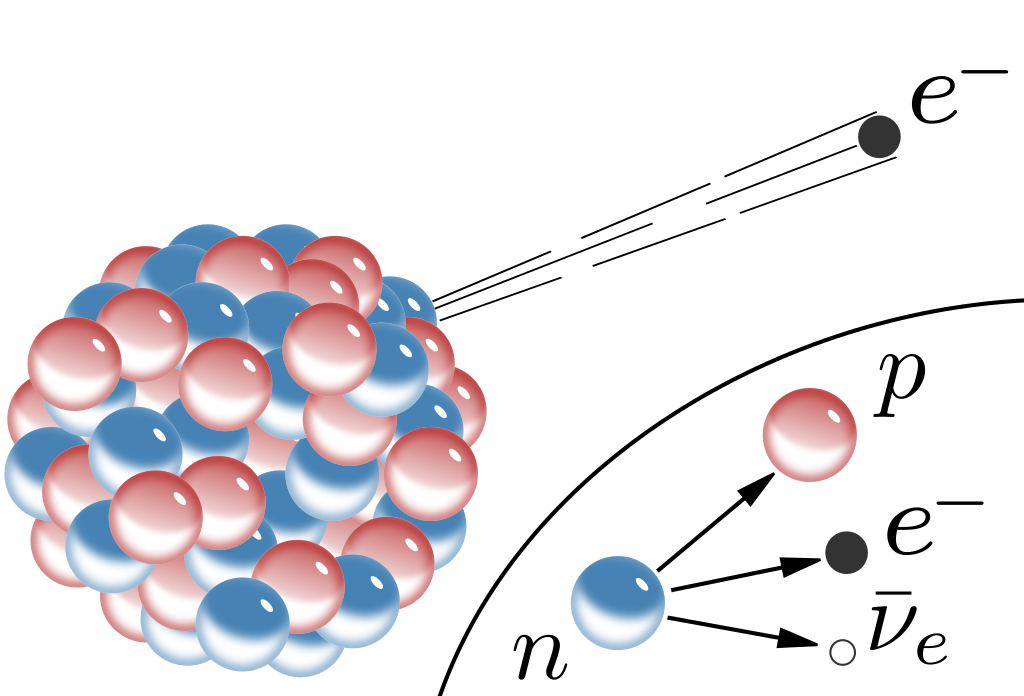
\includegraphics[width=0.9\linewidth,height=0.9\textheight,keepaspectratio]{assets/beta-decay.png}
    \caption*{Beta decay and antineutrino production. Source: Beta\_Decay@Wikipedia}
    \end{figure}


    \end{frame}

    \begin{frame}{What are Neutrinos?}

\begin{minipage}[\textheight]{\textwidth}
\begin{columns}[T]

\begin{column}{0.6\textwidth}
\begin{figure}
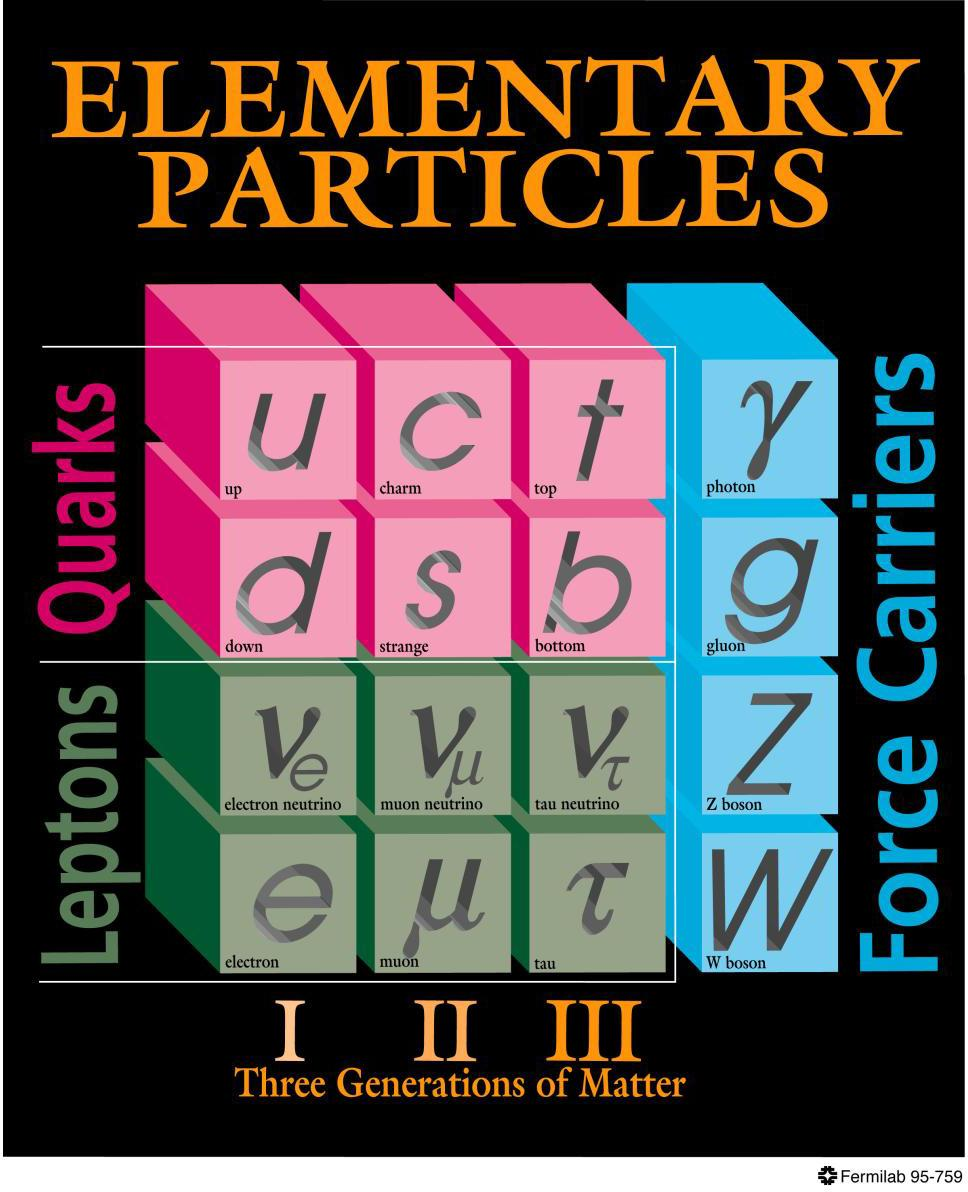
\includegraphics[width=0.9\linewidth,height=0.7\textheight,keepaspectratio]{assets/elementary-particles.jpg}
\caption*{Table of elementary particles. Source: Fermilab} % http://www-d0.fnal.gov/Run2Physics/WWW/results/final/TOP/T06C/T06C.html
\end{figure}
\end{column}

\begin{column}{0.4\textwidth}


    \begin{itemize}
    \item[] Neutrinos are
    \item fermions,
    \item electrically neutral,
    \item light.
    \end{itemize}



\only<1-1>{
\begin{figure}
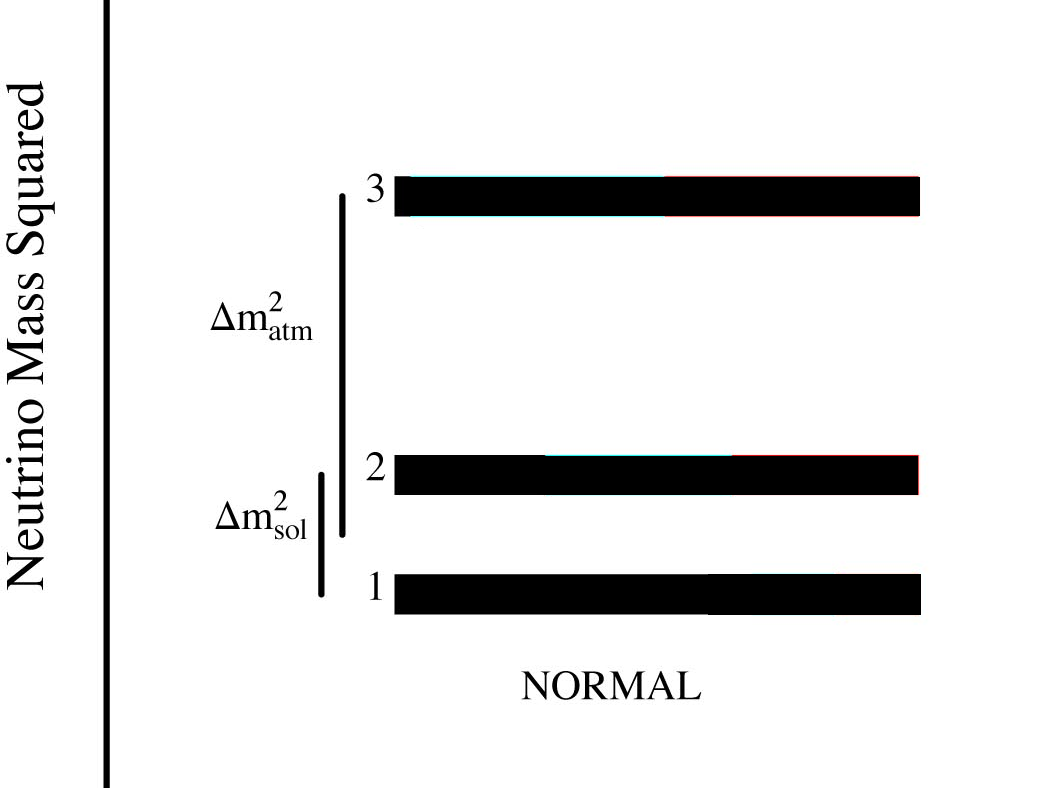
\includegraphics[width=\textwidth]{assets/neutrino-mass-normal-hierarchy-simple.png}
\caption*{Adapted from Olga Mena \& Stephen Parke (2004)}
\end{figure}
}

\only<2-2>{
\begin{figure}
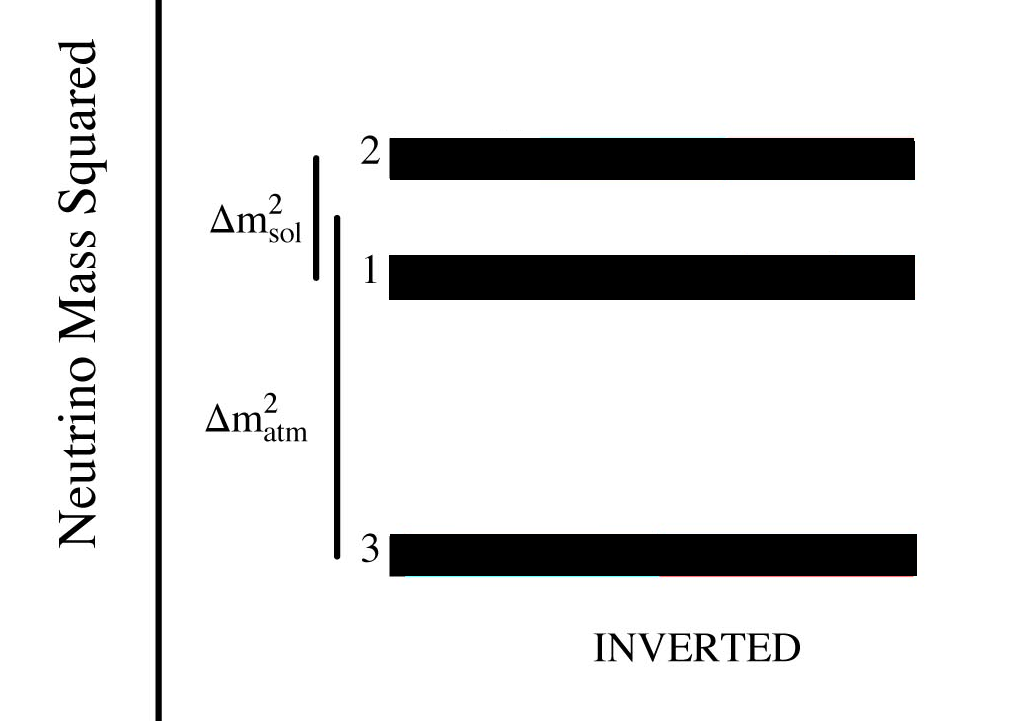
\includegraphics[width=\textwidth]{assets/neutrino-mass-inverted-hierarchy-simple.png}
\caption*{Adapted from Olga Mena \& Stephen Parke (2004)}
\end{figure}
}

\end{column}


\end{columns}
\end{minipage}

\end{frame}

%%%%% Neutrino Oscillations %%%%%%%%%

\subsection{Vacuum Oscillations}


\begin{frame}{What is Neutrino Oscillation?}




\only<1-1>{

\begin{tcolorbox}
\begin{equation*}
  \equalto{\textbf{\large Neutrino Oscillation} }{ \textbf{\large Neutrino Flavor Conversion } }
\end{equation*}

\end{tcolorbox}

\begin{tcolorbox}
\begin{figure}
    \centering
    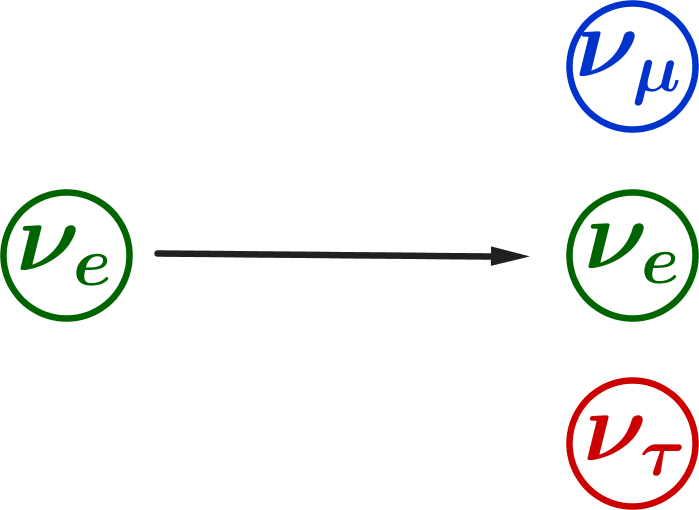
\includegraphics[width=0.6\textwidth]{assets/neutrino-oscillations-illustration}
    \caption*{\color{black}Neutrino Oscillations}
\end{figure}
\end{tcolorbox}

}


\only<2-2>{

\begin{tcolorbox}
\begin{figure}
    \centering
    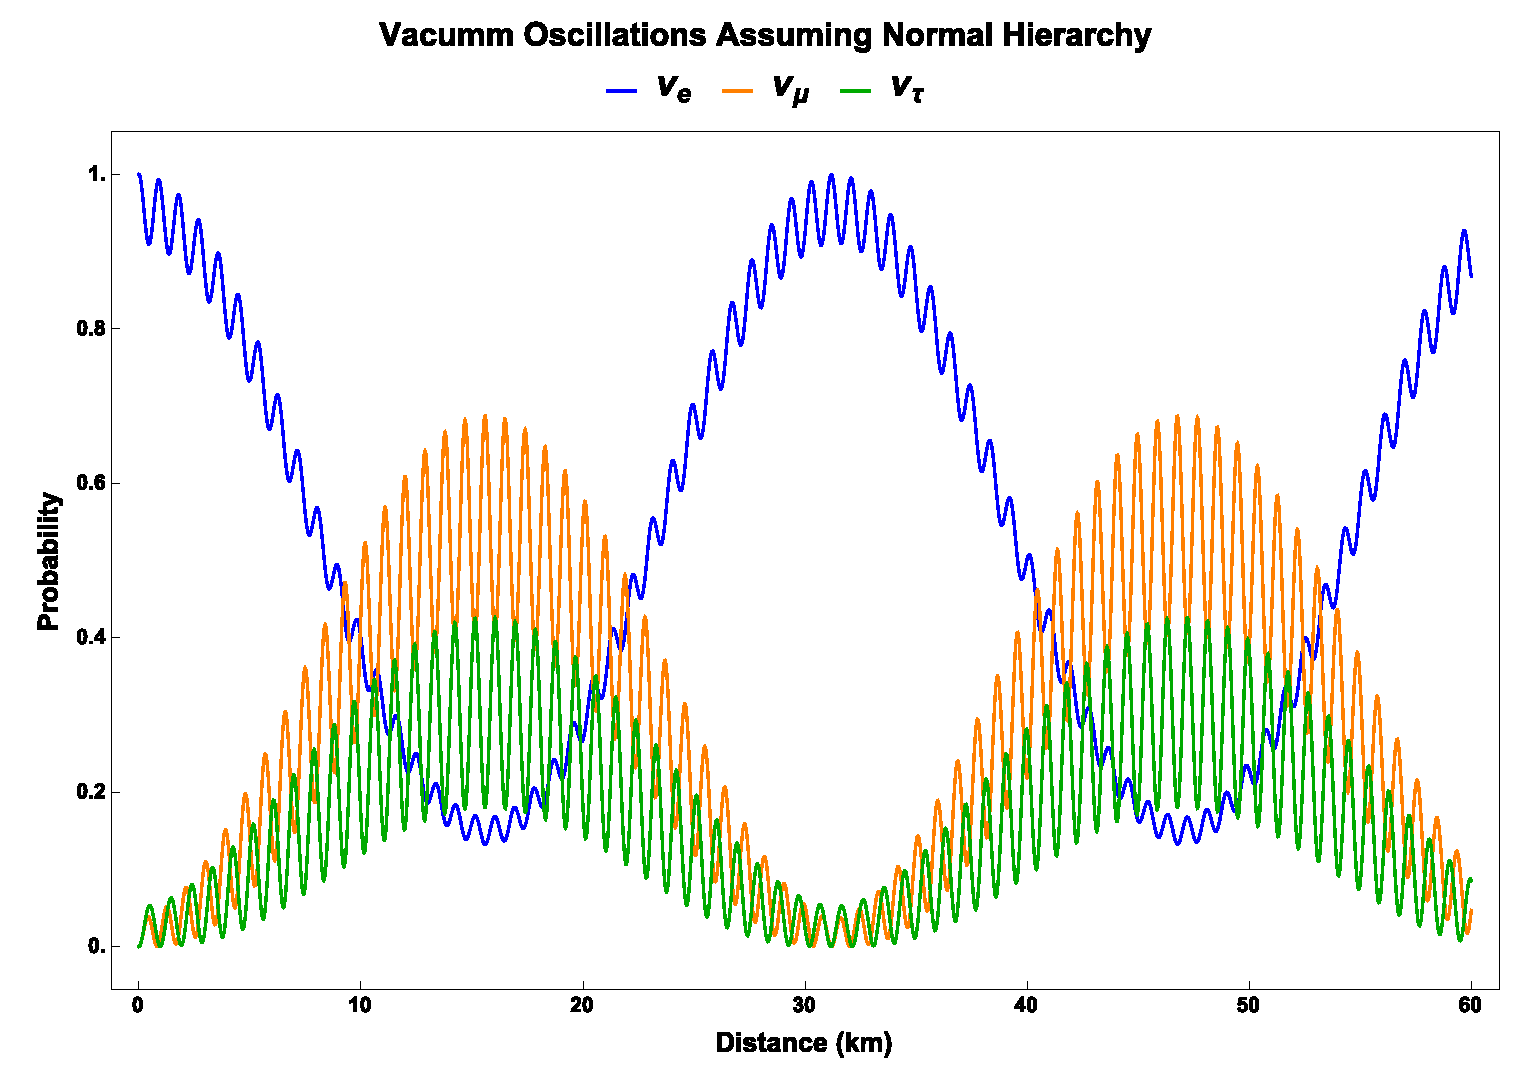
\includegraphics[width=0.9\textwidth]{assets/vacuum-oscillations-3-flavor}
    \caption*{\color{black}Probabilities of finding neutrinos to be in each flavor.}
    %Neutrino energy: 1MeV}
\end{figure}
\end{tcolorbox}

}




\end{frame}


%%%%%% Why Neutrinos Oscillate? %%%%%%%%%

% \subsubsection{Why Do Neutrinos Oscillate}

% For every picture that defines or uses external nodes, you'll have to
% apply the 'remember picture' style. To avoid some typing, we'll apply
% the style to all pictures.
\tikzstyle{every picture}+=[remember picture]

% By default all math in TikZ nodes are set in inline mode. Change this to
% displaystyle so that we don't get small fractions.
\everymath{\displaystyle}


\begin{frame}[fragile]{Why Do Neutrinos Oscillate?}

\begin{tcolorbox}[title=Equation of Motion]

\begin{equation*}
i\partial_x \ket{\Psi} = \hat {\mathbf H} \ket{\Psi}
\end{equation*}

\end{tcolorbox}




\begin{itemize}
\item Basis: Hamiltonian diagonalized basis/mass basis/propagation basis, $\{ \ket{\nu_1}, \ket{\nu_2}\}$.

\item
\begin{equation*}
    \mathbf H = - \frac{\omega_\mathrm v}{2}\boldsymbol{\sigma_3}, \qquad \text{where } \omega_{\mathrm v} = \frac{\delta m^2}{2E}=\frac{m_2^2 - m_1^2}{2E} .
\end{equation*}



\item The system can be solved given initial condition of the amplitudes of the two eigenstates $(\braket{\nu_1}{\Psi(0)},\braket{\nu_2}{\Psi(0)} )^T$,
\begin{equation*}
    \begin{pmatrix}
    \braket{\nu_1}{\Psi(x)} \\
    \braket{\nu_2}{\Psi(x)}
    \end{pmatrix} = \begin{pmatrix}
    \braket{\nu_1}{\Psi(0)} \exp\left( i  \omega_{\mathrm v} x /2 \right) \\
    \braket{\nu_2}{\Psi(0)} \exp\left( -i  \omega_{\mathrm v} x/2 \right)
    \end{pmatrix}
\end{equation*}


\end{itemize}




\end{frame}


%%%%%%%%%

\begin{frame}[fragile]{Why Do Neutrinos Oscillate?}
\setbeamercovered{invisible}

\begin{tcolorbox}[title=Flavor basis]


Neutrino wave function in flavor basis $\{\ket{\nu_{\mathrm e}}, \ket{\nu_{\mathrm \mu}} \}$ is related to state in energy basis $\{\ket{\nu_1},\ket{\nu_2} \}$ through

\begin{equation*}
\begin{pmatrix}\ket{\nu_{\mathrm e}} \\ \ket{\nu_{\mathrm \mu} } \end{pmatrix} = \begin{pmatrix}  \cos\theta_{\mathrm{v}}  & \sin\theta_{\mathrm{v}} \\ -\sin\theta_{\mathrm{v}}  & \cos\theta_{\mathrm{v}} \end{pmatrix}   \begin{pmatrix}\ket{\nu_1} \\ \ket{\nu_2}\end{pmatrix}
\end{equation*}
$\theta_{\mathrm{v}}$: vacuum mixing angle


\end{tcolorbox}

\pause

\begin{tcolorbox}[title=Hamiltonian $\mathbf H$]

\begin{columns}[T] % align columns
\begin{column}{.39\textwidth}

\centering Mass basis
\begin{align*}
&\frac{\omega_{\mathrm{v}}}{2}\begin{pmatrix}
-1  & 0 \\
0 & 1
\end{pmatrix}\\
=&
-\frac{\omega_{\mathrm v} }{2}\boldsymbol{ \sigma_3 }
\end{align*}



\end{column}%
\hfill%

\begin{column}{.59\textwidth}
\centering Flavor basis
\begin{align*}
&\frac{\omega_{\mathrm v} }{2}\begin{pmatrix} -\cos 2\theta_{\mathrm{v}} & \sin 2 \theta_{\mathrm{v}} \\ \sin 2\theta_{\mathrm{v}} & \cos 2\theta_{\mathrm{v}}  \end{pmatrix} \\
=&
\frac{\omega_{\mathrm v} }{2}\left( - \cos 2\theta_{\mathrm{v}}\boldsymbol{ \sigma_3 } + \sin 2\theta_{\mathrm{v}} \boldsymbol{\sigma_1} \right)
\end{align*}

\end{column}%
\end{columns}

\end{tcolorbox}



\end{frame}





\begin{frame}[fragile]{Nature of Neutrino Oscillation}
\setbeamercovered{invisible}



\begin{tcolorbox}[title=Transition Probability]

\begin{equation*}
P(\ket{\nu_{\mathrm e} }\to\ket{\nu_{\mu}})  =  \sin^2(2\theta_{\mathrm v}) \sin^2 \left( \omega_{\mathrm v} x/2 \right)
\end{equation*}

\end{tcolorbox}

\begin{itemize}
    \item $\omega_{\mathrm v}=(m_2^2-m_1^2)/2E$ determines oscillation wavelength.
    \item Mixing angle $\theta_{\mathrm v}$ determines flavor oscillation amplitude.
\end{itemize}



\end{frame}




%%%%%%%%%%%%%%%%%%%%%%%%%%%%%%%%%%%%%%%%%%%%%%%%%%%%%%%%%%%%%%%%%%
%%%%%%%%%%%%%%%%%%%% Matter Effect %%%%%%%%%%%%%%%


\section{Matter Stimulated Oscillations}


\subsection{Matter Interactions, MSW Effect, and Solar Neutrino Problem}


\begin{frame}{Matter Interaction}


% \begin{tcolorbox}[title=PLACEHOLDER]
% SHOULD ADD IN WHY MATTER INTERACTION IS LIKE THIS.
% \end{tcolorbox}

\begin{tcolorbox}
\begin{figure}[ht]
\centering
\begin{minipage}[b]{0.45\linewidth}
\centering
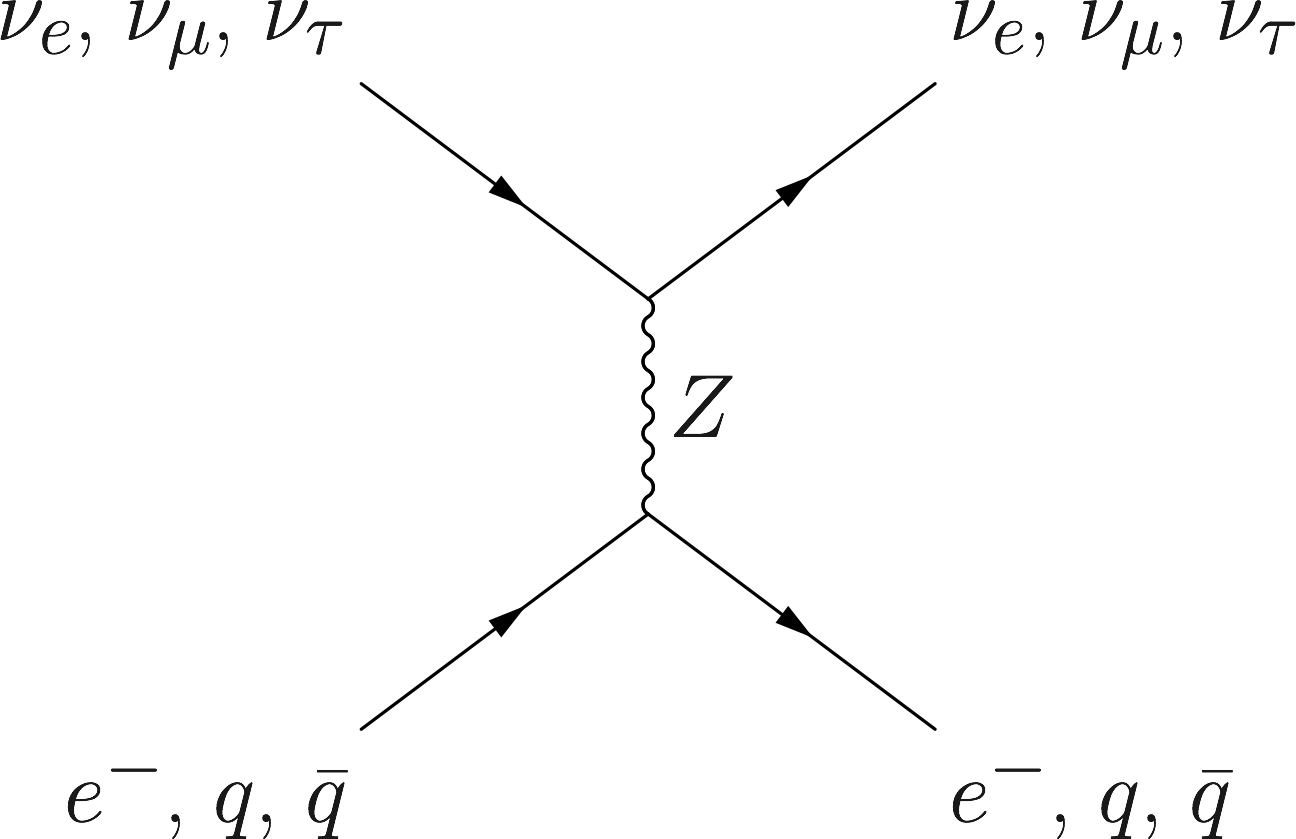
\includegraphics[height=0.32\textheight]{assets/neutral-current.png}
\caption*{\color{black}Neutral current interaction between $\nu_{\mathrm e}$, $\nu_{\mu}$, $\nu_{\tau}$, \\
and $e^{-}$, quarks and antiquarks.}
\end{minipage}%
\begin{minipage}[b]{0.45\linewidth}
\centering
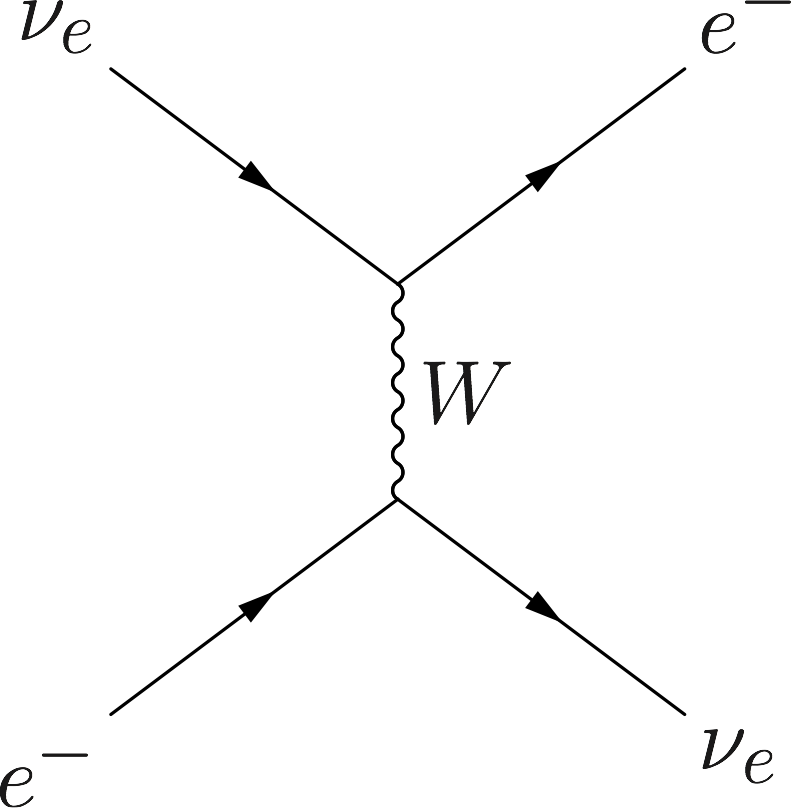
\includegraphics[height=0.32\textheight]{assets/charged-current.png}
\caption*{\\
\color{black}Charged current interaction between $\nu_{\mathrm e}$ and $e^{-}$}
\end{minipage}
\end{figure}

\end{tcolorbox}


\end{frame}





% For every picture that defines or uses external nodes, you'll have to
% apply the 'remember picture' style. To avoid some typing, we'll apply
% the style to all pictures.
\tikzstyle{every picture}+=[remember picture]


% By default all math in TikZ nodes are set in inline mode. Change this to
% displaystyle so that we don't get small fractions.
\everymath{\displaystyle}



\begin{frame}{Matter Interaction}
\setbeamercovered{invisible}

\tikzstyle{na} = [baseline=-.5ex]




\begin{itemize}
    \item[] Hamiltonian with matter interaction in flavor basis  ($\omega_{\mathrm{v}}=\delta m^2/2E$):
        \tikz[na] \node[coordinate] (n1) {};
\end{itemize}


\only<1-1>{
\begin{equation*}
    \mathbf{H} =
    \tikz[baseline]{
            \node[fill=blue!50,anchor=base] (t1)
            {$ \frac{\omega_{\mathrm{v}}}{2}\begin{pmatrix} -\cos 2\theta_{\mathrm{v}} & \sin 2 \theta_{\mathrm{v}} \\ \sin 2\theta_{\mathrm{v}} & \cos 2\theta_{\mathrm{v}}  \end{pmatrix} $}
            }
            \tikz[baseline]{
            \node[fill=red!50, anchor=base] (t2)
            {$
            \pm \sqrt{2}G_{\mathrm{F}} n_{\mathrm{e}}(x) \begin{pmatrix}
            1 & 0 \\
            0 & 0
            \end{pmatrix}
            $};
        }
\end{equation*}



}




\only<2->{
\begin{equation*}
    \mathbf{H} =
    \tikz[baseline]{
            \node[fill=blue!50,anchor=base] (t1)
            {$ \frac{\omega_{\mathrm{v}}}{2}\left( - \cos 2\theta_{\mathrm{v}} \boldsymbol{\sigma_3} + \sin 2\theta_{\mathrm{v}} \boldsymbol{\sigma_1} \right) $}
            }
            \tikz[baseline]{
            \node[fill=red!50, anchor=base] (t2)
            {$
            +\frac{\lambda(x)}{2} \boldsymbol{\sigma_3}
            $};
        }
\end{equation*}

}


\begin{itemize}
    \item Vacuum Hamiltonian
        \tikz[na]\node [coordinate] (n2) {};
    \item Matter interaction
        \tikz[na]\node [coordinate] (n3) {};
    \item<2-> $\lambda(x) = \sqrt{2}G_{\mathrm{F}} n_{\mathrm{e}}(x)$
\end{itemize}





% Now it's time to draw some edges between the global nodes. Note that we
% have to apply the 'overlay' style.
\begin{tikzpicture}[overlay]
        \path[->]<1-> (n2) edge [bend right] (t1);
        \path[->]<1-> (n3) edge [bend right=20] (t2);
\end{tikzpicture}




\end{frame}


%%%%%%%%%%%%%%%%%

% \subsection{MSW Effect}

\begin{frame}{MSW Effect}



\begin{tcolorbox}[title=Hamiltonian in Vacuum]
\begin{equation*}
    \mathbf{H}_{\mathrm{vacuum}}=\frac{\omega_{\mathrm{v}} \cos 2\theta_{\mathrm{v}} }{2} \boldsymbol{\sigma_3} + \frac{ \omega_{\mathrm{v}} \sin 2\theta_{\mathrm{v}}}{2} \boldsymbol{\sigma_1}
\end{equation*}

\end{tcolorbox}
\begin{align*}
    \mathbf{H} &= \frac{\lambda(x) - \omega_{\mathrm{v}} \cos 2\theta_{\mathrm{v}}  }{2}  \boldsymbol{\sigma_3}  + \frac{ \omega_{\mathrm{v}} \sin 2\theta_{\mathrm{v}}}{2}  \boldsymbol{\sigma_1}  \\
    & =\frac{ \omega_{\mathrm{m}}(x)   \cos 2\theta_{\mathrm{m}}(x)  }{2} \boldsymbol{\sigma_3} + \frac{ \omega_{\mathrm{m}}(x)    \sin 2\theta_{\mathrm{m}}(x)  }{2} \boldsymbol{\sigma_1},
\end{align*}
where
\begin{align*}
    \omega_{\mathrm{m}}(x)  = & ~\sqrt{ \left(\lambda(x) - \omega_{\mathrm{v}}\cos 2\theta_{\mathrm{v}} \right)^2 + \omega_{\mathrm{v}}^2 \sin^2 2\theta_{\mathrm{v}}  } ,\\
    \tan 2\theta_{\mathrm{m}}(x)  = & ~\frac{\omega_{\mathrm{v}} \sin 2\theta_{\mathrm{v}}  }{ \omega_{\mathrm{v}}\cos 2\theta_{\mathrm{v}} - \lambda(x)  }.
\end{align*}




\end{frame}


\begin{frame}{MSW Effect}

Constant matter profile $\lambda_0$ as an example,

\begin{tcolorbox}[title=Significance of $\theta_{\mathrm{m}}$]

Define matter basis $\{\ket{\nu_{\mathrm{L}}}, \ket{\nu_{\mathrm{H}}}\}$

\begin{equation*}
\begin{pmatrix}
\ket{\nu_{\mathrm{e}}} \\
\ket{\nu_{\mu}}
\end{pmatrix} =
\begin{pmatrix}
\cos\theta_{\mathrm m} & \sin\theta_{\mathrm m} \\
-\sin\theta_{\mathrm m} & \cos\theta_{\mathrm m}
\end{pmatrix}\begin{pmatrix}
\ket{\nu_{\mathrm{L}}} \\
\ket{\nu_{\mathrm{H}}}
\end{pmatrix}
\end{equation*}

\end{tcolorbox}


In matter basis

\begin{equation*}
    \mathbf{H}_{\text{matter-basis}} = -\frac{\omega_{\mathrm m}}{2}\boldsymbol{\sigma_3}
\end{equation*}


\end{frame}


\begin{frame}{MSW Resonance}


% \begin{tcolorbox}[title=Hamiltonian with Matter Potential]
\begin{align*}
    \mathbf{H} &= \frac{\lambda(x) -\omega_{\mathrm{v}} \cos 2\theta_{\mathrm{v}} }{2} \boldsymbol{\sigma_3}  + \frac{ \omega_{\mathrm{v}} \sin 2\theta_{\mathrm{v}}}{2}  \boldsymbol{\sigma_1} \\
    &=\frac{ \omega_{\mathrm{m}}(x)    \cos 2\theta_{\mathrm{m}}(x)  }{2} \boldsymbol{\sigma_3} + \frac{ \omega_{\mathrm{m}}(x)    \sin 2\theta_{\mathrm{m}}(x)  }{2} \boldsymbol{\sigma_1}
\end{align*}
%
\begin{equation*}
\tan 2\theta_{\mathrm{m}}(x) =  \frac{\omega_{\mathrm{v}} \sin 2\theta_{\mathrm{v}}  }{ \omega_{\mathrm{v}}\cos 2\theta_{\mathrm{v}} - \lambda(x)  }.
\end{equation*}
%
\begin{equation*}
\begin{pmatrix}
\ket{\nu_{\mathrm{e}}} \\
\ket{\nu_{\mu}}
\end{pmatrix} =
\begin{pmatrix}
\cos\theta_{\mathrm m} & \sin\theta_{\mathrm m} \\
-\sin\theta_{\mathrm m} & \cos\theta_{\mathrm m}
\end{pmatrix}\begin{pmatrix}
\ket{\nu_{\mathrm{L}}} \\
\ket{\nu_{\mathrm{H}}}
\end{pmatrix}
\end{equation*}


% \end{tcolorbox}





\begin{tcolorbox}[title=Transition Probability]
\begin{equation*}
P(\ket{\nu_{\mathrm{e}}}\to\ket{\nu_\mu})  =  \sin^2(2\theta_{\mathrm{m}}) \sin^2 \left( \omega_{\mathrm{m}} x \right)
\end{equation*}

\end{tcolorbox}





\end{frame}



%%%%%%% MSW Effect %%%%%%%%%

%\subsubsection{Solar Neutrino Problem}

\begin{frame}{Solar Neutrino Problem}


\begin{figure}
    \centering
    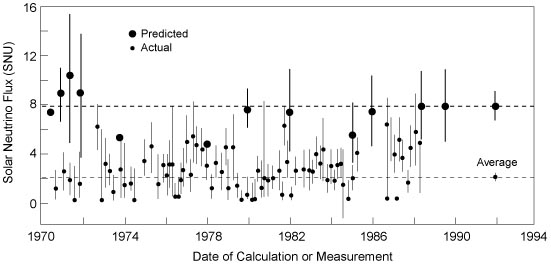
\includegraphics[width=0.9\textwidth]{assets/chlorine-detector-solar-neutrinos.jpg} %https://ase.tufts.edu/cosmos/print_images.asp?id=37
    %https://ase.tufts.edu/cosmos/view_picture.asp?id=585
    \caption*{Chlorine detector (Homestake experiment) results and theory predictions. SNU: 1 event for $10^{36}$ target atoms per second. Kenneth R. Lang (2010)}
\end{figure}


\end{frame}


\begin{frame}{MSW Effect and Solar Neutrinos}

% \setbeamercovered{invisible}



\begin{equation*}
    \mathbf{H} = \frac{\lambda(x) - \omega_{\mathrm v} \cos 2\theta_{\mathrm v}}{2} \boldsymbol{\sigma_3} + \frac{ \omega_{\mathrm v} \sin 2\theta_{\mathrm v}}{2} \boldsymbol{\sigma_1}
\end{equation*}


\begin{equation*}
\begin{pmatrix}
\ket{\nu_{\mathrm{L}}} \\
\ket{\nu_{\mathrm{H}}}
\end{pmatrix} =
\begin{pmatrix}
\cos\theta_{\mathrm m} & -\sin\theta_{\mathrm m} \\
\sin\theta_{\mathrm m} & \cos\theta_{\mathrm m}
\end{pmatrix}\begin{pmatrix}
\ket{\nu_{\mathrm{e}}} \\
\ket{\nu_{\mu}}
\end{pmatrix}
\end{equation*}


\begin{equation*}
    \mathbf{H}_{\text{matter-basis}} = -\frac{\omega_{\mathrm m}}{2}\boldsymbol{\sigma_3}
\end{equation*}



\begin{figure}
\centering
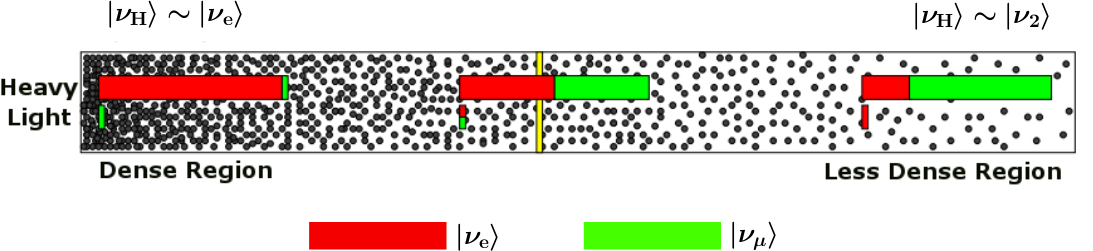
\includegraphics[width=0.9\textwidth]{assets/msw-and-density.png}
\caption*{Yellow bar is the resonance point. Red: $\ket{\nu_e}$. Green: $\ket{\nu_\mu}$. Adapted from Smirnov, 2003.}
\end{figure}



\end{frame}






\begin{frame}{MSW Effect}


Suppose $\omega_{\mathrm v} = (m_2^2 - m_1^2)/2E <0$,

\begin{equation*}
    \mathbf{H} = \colorbox{blue!50}{$
    -\frac{\omega_{\mathrm{v}}}{2}\begin{pmatrix} -\cos 2\theta_{\mathrm{v}} & \sin 2 \theta_{\mathrm{v}} \\ \sin 2\theta_{\mathrm{v}} & \cos 2\theta_{\mathrm{v}}  \end{pmatrix}
    $}
             \colorbox{red!50}{$
            + \sqrt{2}G_{\mathrm{F}} n_{\mathrm{e}}(x) \begin{pmatrix}
            1 & 0 \\
            0 & 0
            \end{pmatrix}
            $}
\end{equation*}

\centering
$\big\downarrow$

\begin{equation*}
    \mathbf{H} =
    \left(
    %\colorbox{blue!20}{$
     \frac{-\omega_{\mathrm{v}}}{2} \cos 2\theta_{\mathrm{v}}
    % $} \colorbox{red!20}{$
    + \frac{\lambda(x)}{2}
    % $}
    \right) \boldsymbol{\sigma_3}
    % \colorbox{blue!20}{$
            - \frac{\omega_{\mathrm v}}{2}\sin 2\theta_{\mathrm v} \boldsymbol{\sigma_1}
     %       $}
\end{equation*}

\end{frame}


%%%%%%%%%%%%%%%%%%%%%%%%%%%%%%%%%%%%%%%%%%%%%%%%%%%%%%%%%%%%%%%%%%
%%%%%%%%%%%%%%%%%%%% Stimulated Effect/Multi-frequency stimulation %%%%%%%%%%%%%%%
\subsection{Stimulated Neutrino Oscillations and Rabi Oscillations}

\begin{frame}{Supernova Matter Density Profile}

\begin{tcolorbox}[title=Why Do We Care]

Astrophysical environments: supernovae, accretion disks etc

\end{tcolorbox}

\begin{figure}
    \centering
    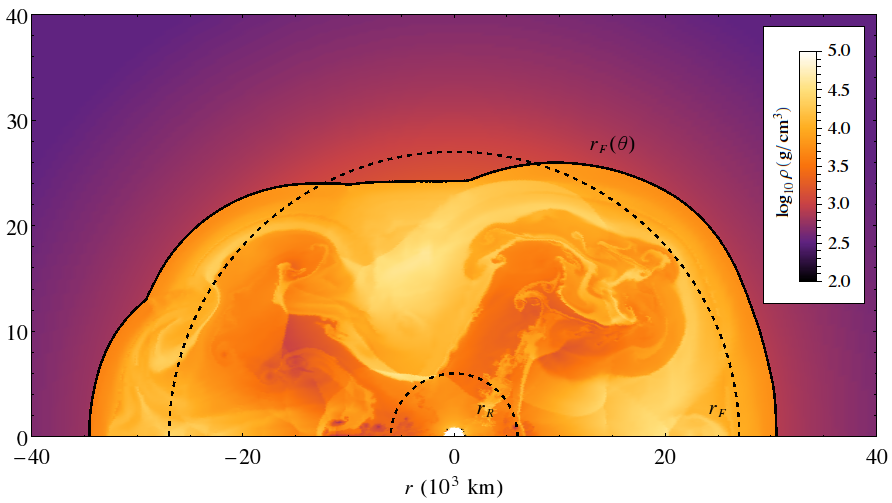
\includegraphics[height=0.5\textheight]{assets/supernova-shock-turbulence.png}
    \caption*{Supernova shock and turbulence. E. Borriello, et al  (2014)}
    %https://inspirehep.net/record/1262293?ln=en
    % arXiv: 1310.7488
\end{figure}

\vspace{-1em}
\begin{equation*}
\Delta n_e (r) = \sum_n c_n \sin( k_n r + \phi_n )
\end{equation*}


\end{frame}










\begin{frame}{Stimulated Neutrino Oscillations}


\only<1-1>{
% Matter profile
\begin{tcolorbox}[title=Matter Profile]
\begin{equation*}
    \lambda(x)  = \lambda_0 + {\color{red}\delta\lambda(x)}
\end{equation*}
\end{tcolorbox}


% Basis


\begin{tcolorbox}[title=Basis]

Background matter basis: Hamiltonian is diagonalized with only background matter profile $\lambda_0$,

\begin{equation*}
    \mathrm{H}_{\mathrm{background}} = -\frac{\omega_{\mathrm{m}}}{2} \boldsymbol{\sigma_3}.
\end{equation*}

\end{tcolorbox}


% Hamiltonian of with perturbation in matter profile, in background matter basis
\begin{tcolorbox}[title=Hamiltonian]

\begin{equation*}
    \mathbf H = \frac{1}{2}\left( - \omega_{\mathrm{m}} + {\color{red}\delta \lambda(x)} \cos 2\theta_{\mathrm{m}} \right) \boldsymbol{\sigma_3} - \frac{{\color{red}\delta \lambda(x) } }{2} \sin \theta_{\mathrm{m}} \boldsymbol{\sigma_1}.
\end{equation*}


\end{tcolorbox}

}

\only<2-2>{

% \begin{tcolorbox}
% Kneller, J. P., McLaughlin, G. C., \& Patton, K. M. (2013). J. Phys. G: Nucl. Part. Phys. {\bf{40}} (2013) 055002.
% \end{tcolorbox}

\begin{tcolorbox}
P. Krastev and A. Smirnov (1989); J. Kneller et al (2013);\\ K. Patton et al (2014);
\end{tcolorbox}


\begin{figure}
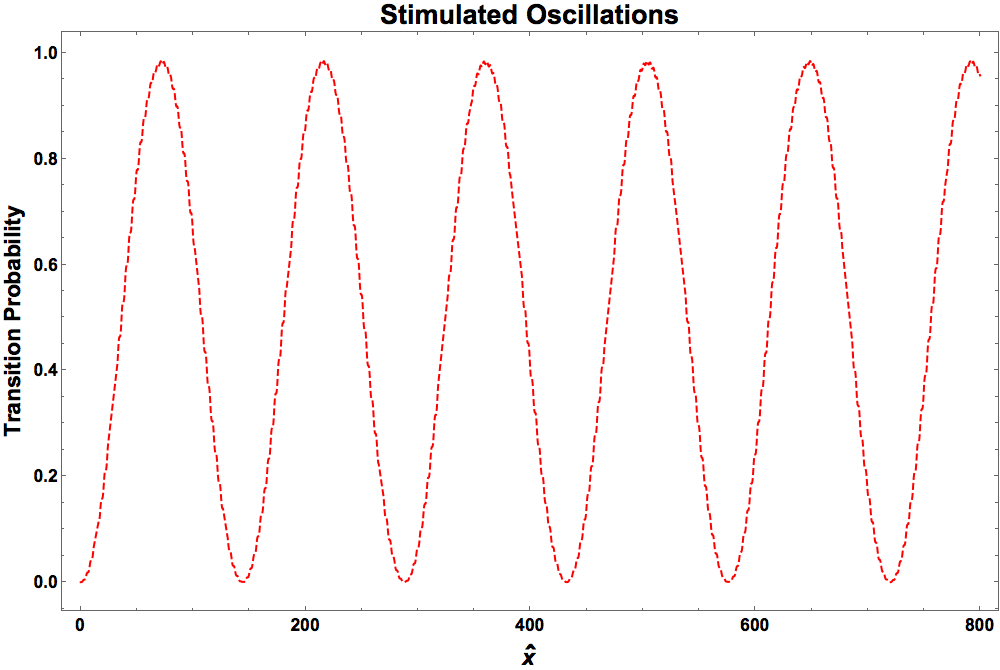
\includegraphics[width=0.8\textwidth]{assets/stimulated-oscillation-phenomenon.png}
%stimulated-neutrino-oscillations-kneller.png}
\caption*{Stimulated oscillations. $\lambda(x) = \lambda_0 +  A \sin (k x)$  with $\hat x = \omega_{\mathrm m} x $, $A=0.1\omega_{\mathrm m}$, $k=0.995\omega_{\mathrm m}$, $\theta_{\mathrm{m}}=\pi/6$}
\end{figure}


}





\end{frame}




















%%%%%%%%%%%%%%%%%%%%%%%%%%%%%%%%
% Intuitive Demonstration BEGIN
%%%%%%%%%%%%%%%%%%%%%%%%%%%%%%%%


\begin{frame}{Hamiltonian, and Basis, and Rabi Oscillations}



\begin{tcolorbox}[title=Hamiltonian in Background Matter Basis]
    \begin{equation*}
    \mathbf {H} = \frac{1}{2}\left( - \omega_{\mathrm{m}} + {\color{red}\delta \lambda(x)} \cos 2\theta_{\mathrm{m}} \right) \sigma_3 - \frac{  {\color{red}\delta \lambda(x)}  }{2} \sin 2\theta_{\mathrm{m}} \sigma_1.
\end{equation*}
\end{tcolorbox}


Matter profile
\begin{equation*}
    \lambda(x) = \lambda_0 + {\color{red}A \cos (k x)},
\end{equation*}


\begin{equation*}
    \mathbf {H} = \frac{1}{2}\left( - \omega_{\mathrm{m}} +  \cos 2\theta_{\mathrm{m}}{\color{red}A\cos(kx)} \right) \sigma_3 - \frac{  \sin 2\theta_{\mathrm{m} }  }{2}{\color{red}A \cos(kx)}  \sigma_1.
\end{equation*}





\end{frame}




\begin{frame}{Hamiltonian, and Basis, and Rabi Oscillations}





\only<1->{

\begin{columns}[T]
\begin{column}{0.5\textwidth}
\begin{tcolorbox}[title=Rabi Oscillation]

Hamiltonian
\begin{equation*}
    -\frac{\omega_0}{2} \sigma_3 - \frac{\alpha}{2} \begin{pmatrix}
    0 & e^{ikt}\\
    e^{-ikt} & 0
    \end{pmatrix}
\end{equation*}
\end{tcolorbox}

\end{column}%
\begin{column}{0.5\textwidth}
\begin{figure}
    \centering
    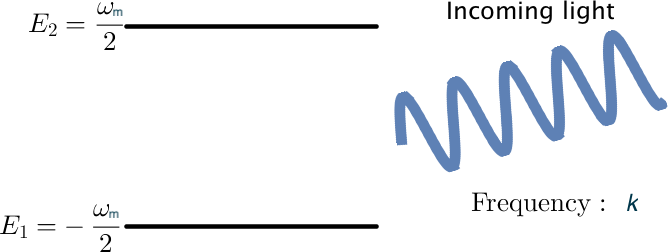
\includegraphics[width=\textwidth]{assets/rabi-diagram.png}
\end{figure}


\end{column}
\end{columns}

}


\only<2>{
\begin{textblock*}{10pt}(160pt,1pt)
\tiny
\begin{equation*}
  \frac{1}{2}\left( - \omega_{\mathrm{m}} +  \cos 2\theta_{\mathrm{m}}{\color{red}A\cos(kx)} \right) \sigma_3 - \frac{  \sin 2\theta_{\mathrm{m} }  }{2}{\color{red}A \cos(kx)}  \sigma_1
\end{equation*}
\end{textblock*}


The transition probability from low energy to high energy is

\begin{equation*}
    P_{1\to 2} = \frac{\colorbox{red!50}{$\alpha$}^2}{\colorbox{red!50}{$\alpha$}^2+(\colorbox{blue!50}{$\omega_0 - k$})^2} \sin^2 \left( \frac{\Omega_{\mathrm R}}{2} t \right),
\end{equation*}
where
\begin{equation*}
\Omega_{\mathrm R} = \sqrt{\colorbox{red!50}{$\alpha$}^2+(\colorbox{blue!50}{$\omega_0 - k$})^2}
\end{equation*}
is Rabi frequency.

}

\only<3>{

The transition probability from low energy to high energy is
\begin{equation*}
    P_{1\to 2} = \frac{1}{1 + D^2} \sin^2 \left( \frac{\Omega_{\mathrm R}}{2} t \right),
\end{equation*}
where
\begin{equation*}
    D = \left\vert\frac{\omega_0 - k}{\alpha} \right\vert.
\end{equation*}

}


\end{frame}


\begin{frame}{Visualizing Rabi Oscillations}

\begin{textblock*}{10pt}(250pt,1pt)
\small
\begin{equation*}
  % The Pauli matrices form
  %-\frac{\omega_0}{2} \sigma_3 - \frac{\alpha}{2} \cos(kt)\sigma_1 + \frac{\alpha}{2}\sin(kt)\sigma_2
  % The single matrix form
   -\frac{\omega_0}{2} \sigma_3 - \frac{\alpha}{2} \begin{pmatrix}
    0 & e^{ikt}\\
    e^{-ikt} & 0
    \end{pmatrix}
\end{equation*}
\end{textblock*}



\begin{columns}[T]
\begin{column}{0.6\textwidth}

\begin{align*}
    &-\frac{\omega_0}{2} \sigma_3 - \frac{\alpha}{2} \cos(kt) \sigma_1 + \frac{\alpha}{2}\sin(kt) \sigma_2 \\
= & \begin{pmatrix}
\alpha \cos(kt) &
-\alpha \sin(kt) &
\omega_0
\end{pmatrix}
\colorbox{blue!50}{$\begin{pmatrix}
-\sigma_1/2 \\
-\sigma_2/2 \\
-\sigma_3/2
\end{pmatrix}
$} \\
=& \vec H \cdot (-\vec{\sigma}/2)
\end{align*}

\end{column}%
\begin{column}{0.4\textwidth}
\begin{figure}
    \centering
    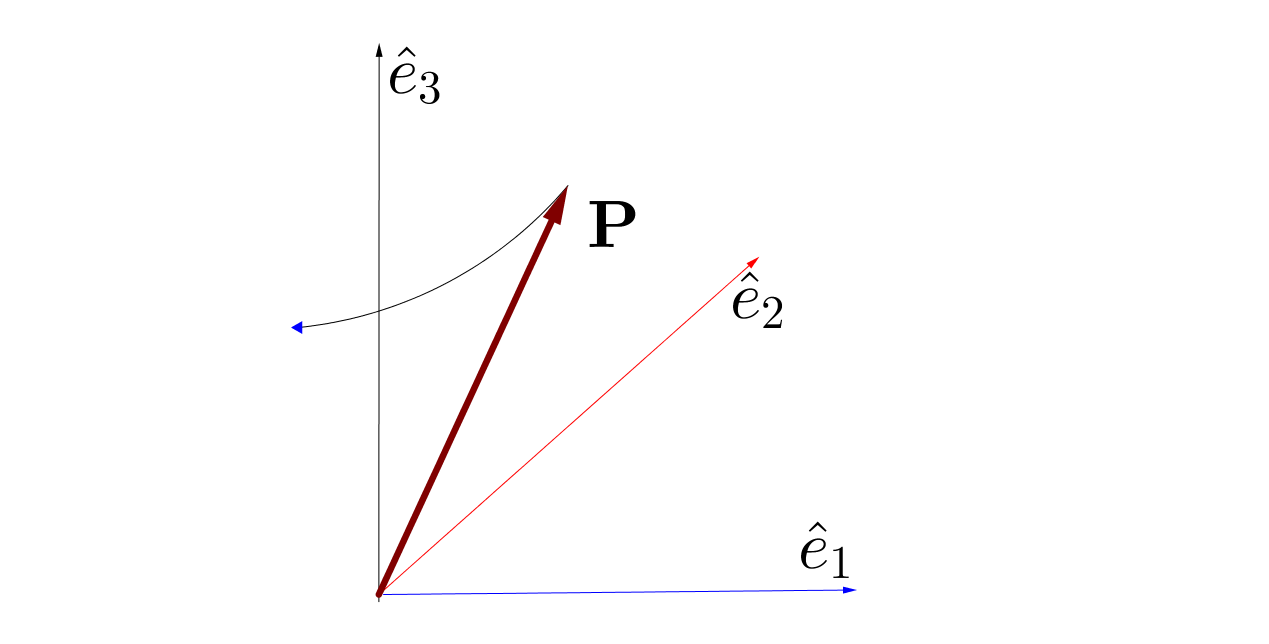
\includegraphics[width=\textwidth,trim={2cm 0 3cm 0},clip]{assets/rabi-bloch-vector-rotation}
\end{figure}


\end{column}
\end{columns}


\begin{equation*}
    D = \left\vert\frac{\omega_0 - k}{\alpha} \right\vert
\end{equation*}

is

\end{frame}

\begin{frame}{Interferences of Rabi Oscillations}

\begin{textblock*}{10pt}(250pt,16pt)
\small
\begin{equation*}
\begin{pmatrix}
0\\
0\\
\omega_0
\end{pmatrix} +  \alpha\begin{pmatrix}
 \cos(kt) \\
- \sin(kt) \\
0
\end{pmatrix}
\end{equation*}
\end{textblock*}


\begin{align*}
    \mathbf {H} =& \frac{1}{2}\left( - \omega_{\mathrm{m}} \colorbox{gray!70}{$+  \cos 2\theta_{\mathrm{m}}A\cos(kx) $} \right) \sigma_3 - \frac{  \sin 2\theta_{\mathrm{m} }  }{2}A \cos(kx)  \sigma_1\\
    \to& -\frac{\omega_m}{2} \sigma_3 - \frac{A\sin 2\theta_{\mathrm m}}{2} \cos(kx)\sigma_1
\end{align*}

\begin{equation*}
    \vec H = \begin{pmatrix}
    0\\
    0\\
    \omega_m
    \end{pmatrix} + \frac{A\sin 2\theta_{\mathrm m}}{2}\begin{pmatrix}
     \cos(kx)\\
    -\sin(kx)\\
    0
    \end{pmatrix} + \frac{A\sin 2\theta_{\mathrm m}}{2}\begin{pmatrix}
    \cos(-kx)\\
    -\sin(-kx)\\
    0
    \end{pmatrix}
\end{equation*}

\begin{tcolorbox}
\centering
Two frequencies!
\end{tcolorbox}


\end{frame}





\begin{frame}{Interferences of Rabi Oscillations}


\begin{equation*}
    \vec H = \begin{pmatrix}
    0\\
    0\\
    \omega_m
    \end{pmatrix} + \alpha_1\begin{pmatrix}
     \cos(k_1x)\\
    -\sin(k_1x)\\
    0
    \end{pmatrix} + \colorbox{blue!50}{$\alpha_2\begin{pmatrix}
    \cos(k_2x)\\
    -\sin(k_2x)\\
    0
    \end{pmatrix}$}
\end{equation*}

Co-rotating frame of the second frequency,



\begin{equation*}
    \vec H = \begin{pmatrix}
    0\\
    0\\
    \omega_m - k_2
    \end{pmatrix} + \alpha_1\begin{pmatrix}
     \cos(k_1-k_2x)\\
    -\sin(k_1-K_2x)\\
    0
\end{pmatrix} + \colorbox{blue!50}{$\alpha_2\begin{pmatrix}
    1\\
    0\\
    0
    \end{pmatrix}$}
\end{equation*}




\end{frame}



\begin{frame}{Rabi Formula Works}


\begin{figure}
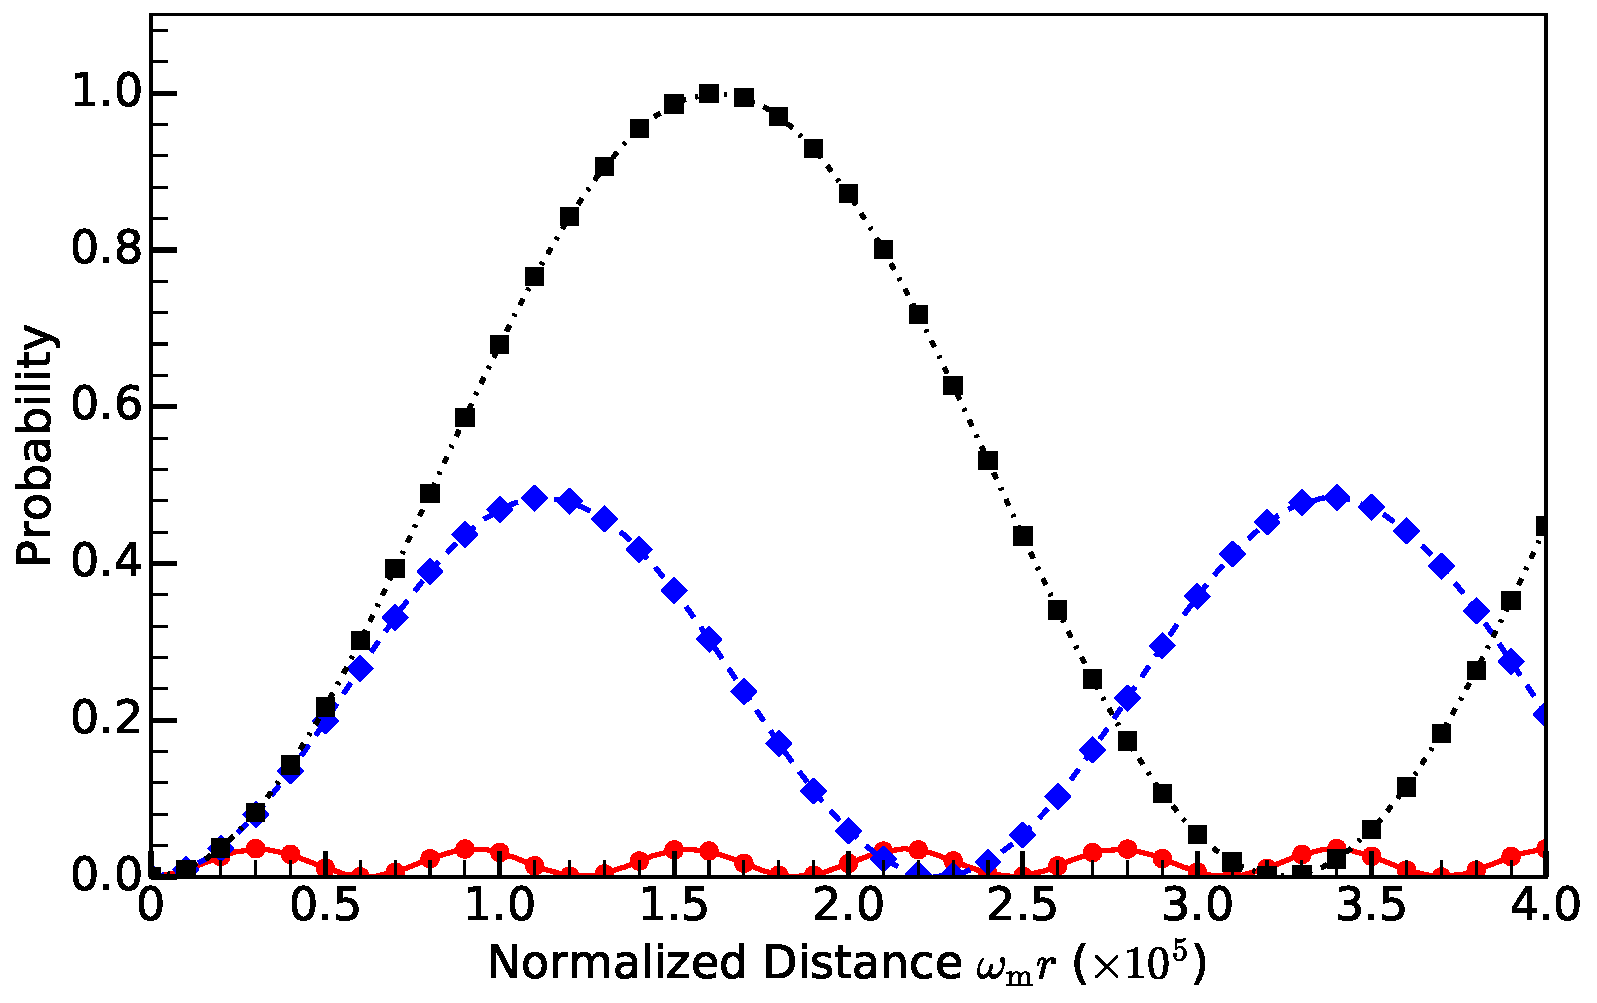
\includegraphics[width=0.9\textwidth]{assets/rabiOscillationsNeutrinoCoincidence-single-frequency}
%stimulated-neutrino-oscillations-kneller.png}
\caption*{
Dots, diamonds, triangles, and squares are for $k=\omega_{\mathrm m}$, $k=(1-2\times 10^{-5})\omega_{\mathrm m}$, and $k=(1-10^{-4})\omega_{\mathrm m}$ respectively.\\
Lines: Rabi formula
}
\end{figure}


\end{frame}

%%%%%%%%%%%%%%%%%%%%%%%%%%%%%%%%
% Intuitive Demonstration END
%%%%%%%%%%%%%%%%%%%%%%%%%%%%%%%%


%\subsubsection{Interferences of Rabi Oscillations}



\begin{frame}{Interferences of Rabi Oscillations}

Matter profile with two frequencies,

\begin{equation*}
    \lambda(x) = \lambda_0  + \frac{\alpha_1}{2}\sin(k_1 x) \sigma_1
\end{equation*}

\end{frame}







\begin{frame}{Understanding Stimulated Oscillations}


Matter profile
\begin{equation*}
    \lambda(x) = \lambda_0 + {\color{red}A \sin (k x)},
\end{equation*}


\begin{tcolorbox}[title=Hamiltonian in Background Matter Basis]
\vspace{-0.5em}
    \begin{equation*}
    \mathbf {H} = \frac{1}{2}\left( - \omega_{\mathrm{m}} + {\color{red}\delta \lambda(x)} \cos 2\theta_{\mathrm{m}} \right) \boldsymbol{\sigma_3} - \frac{  {\color{red}\delta \lambda(x)}  }{2} \sin \theta_{\mathrm{m}} \boldsymbol{\sigma_1}.
\end{equation*}
\end{tcolorbox}


\begin{tcolorbox}[title=A Better Basis]


Define new basis \{$\ket{\tilde\nu_{\mathrm{L} }}$,$\ket{\tilde\nu_{\mathrm{H} }}$\} is related to background matter basis \{$\ket{\nu_{\mathrm{L} }}$,$\ket{\nu_{\mathrm{H} }}$\} through
\begin{equation*}
    \begin{pmatrix}
    \ket{\nu_{\mathrm{L} }} \\
    \ket{\nu_{\mathrm{H} }}
    \end{pmatrix} = \begin{pmatrix}
     e^{-i \eta (x)} & 0 \\  0 & e^{i \eta (x)}
    \end{pmatrix}\begin{pmatrix}
    \ket{\tilde\nu_{\mathrm{L} }}\\
    \ket{\tilde\nu_{\mathrm{H} }}
    \end{pmatrix},
\end{equation*}
where
\begin{equation*}
    \eta(x) - \eta(0) = - \frac{\omega_{\mathrm{m}}}{2} x + \frac{\cos 2\theta_{\mathrm{m}}}{2} \int_0^x {\color{red}\delta\lambda (\tau)} d\tau.
\end{equation*}

\end{tcolorbox}



\end{frame}






% \subsubsection{Single Frequency Matter Profile}



\begin{frame}{Single Frequency Matter Profile}


Hamiltonian in new basis
\begin{equation*}
    \mathbf{\widetilde H} = - \frac{ {\color{red}\delta \lambda(x)}  }{2} \sin 2\theta_{\mathrm{m}} \begin{pmatrix} 0 & e^{2i\eta(x)} \\ e^{-2 i\eta(x) } & 0 \end{pmatrix} = \begin{pmatrix}
    0 & h \\
    h^* & 0
    \end{pmatrix}
\end{equation*}


\begin{tcolorbox}[title=Hamiltonian in New Basis]

\begin{align*}
    h &\equiv -\frac{ {\color{red}\delta \lambda(x)}  }{2} e^{2i\eta(x)} \\
    & = \frac{i}{4}\left[ \exp\left(i(k + \omega_{\mathrm m})x + i\cos 2\theta_{\mathrm m} \frac{A}{k} \cos (k x ) \right) \right. \\
    &\phantom{=} \left. - \exp\left(i(-k  + \omega_{\mathrm m})x + i\cos 2\theta_{\mathrm m} \frac{A}{k} \cos (k x ) \right) \right]
\end{align*}


\end{tcolorbox}




\end{frame}




\begin{frame}{Rabi Oscillations}

\only<1>{
\begin{figure}
    \centering
    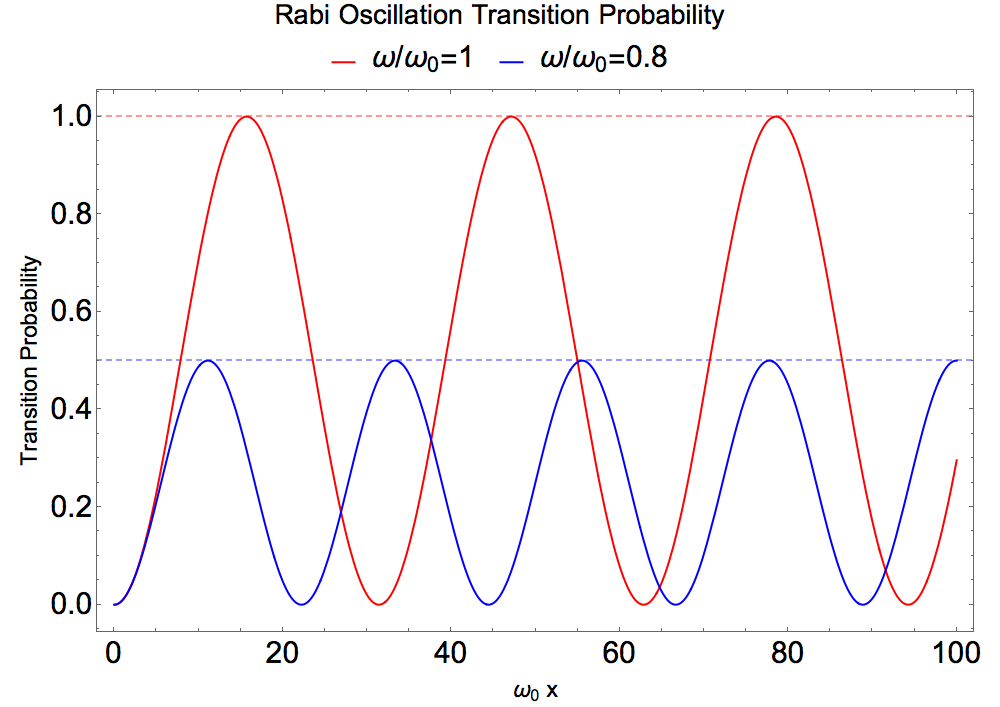
\includegraphics[width=0.9\textwidth]{assets/rabi-oscillations.png}
    \caption*{}
\end{figure}

}

\only<2->{
\begin{figure}
    \centering
    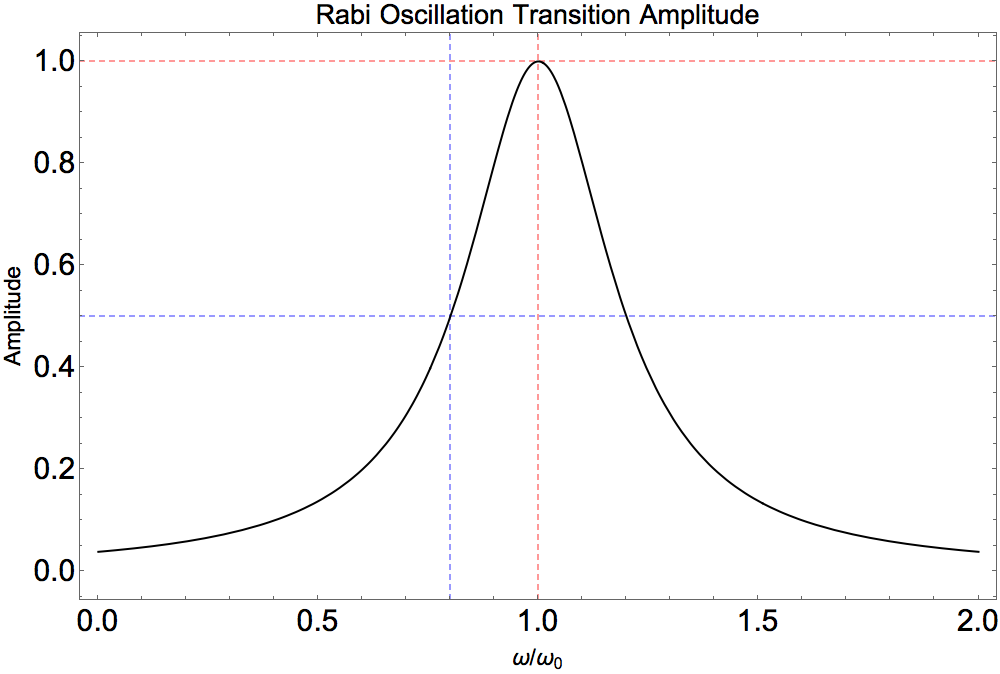
\includegraphics[width=0.9\textwidth]{assets/rabi-resonance.png}
    \caption*{Resonance}
\end{figure}
}


\end{frame}




\begin{frame}{Single Frequency Matter Profile}







\begin{tcolorbox}[title=Off-diagonal Term in Our System]

\begin{equation*}
    \mathbf{\widetilde H}= \begin{pmatrix}
    0 & h \\
    h^* & 0
    \end{pmatrix}
\end{equation*}

\begin{align*}
    h & \propto \left[ \exp\left(i(k + \omega_{\mathrm m})x + i\cos 2\theta_{\mathrm m} \frac{A}{k} \cos (k x ) \right) \right. \\
    &\phantom{\propto} \left. - \exp\left(i(-k  + \omega_{\mathrm m})x + i\cos 2\theta_{\mathrm m} \frac{A}{k} \cos (k x ) \right) \right]
\end{align*}

\end{tcolorbox}




Jacobi-Anger expansion

\begin{equation*}
e^{i \beta \cos ( k x)} = \sum_{n=-\infty}^\infty i^n J_n(\beta) e^{i n k x},
\end{equation*}

where $J_n(\beta)$ are Bessel's functions of the first kind.


\end{frame}




\begin{frame}{Single Frequency Matter Profile}

\only<1-1>{
\begin{tcolorbox}[title=Scaled Quantities]
Characteristic scale: $\omega_{\mathrm{m}}$



\begin{itemize}
\item \color{black}$\hat A = A/\omega_{\mathrm{m}}$
    \item \color{black} $\hat k = k/\omega_{\mathrm{m}}$
    \item \color{black} $\hat x = \omega_{\mathrm{m}} x$
    \item \color{black} $\hat h= h/\omega_{\mathrm{m}}$
\end{itemize}
\end{tcolorbox}
}



\only<2-2>{
\begin{tcolorbox}[title=Rotation Wave Approximation]

The off-diagonal element of Hamiltonian
\begin{equation*}
\mathbf{\widetilde H}= \sum_{n=-\infty}^{\infty} \begin{pmatrix}
0 & \frac{1}{2} \hat B_n e^{i  {\color{blue} (n\hat k-1) } \hat x}\\
\frac{1}{2} \hat B_n^* e^{ -i  {\color{blue} (n\hat k-1) } \hat x} & 0
\end{pmatrix}
\end{equation*}


where $\hat B_n =  - (-i)^n  n \hat k \tan 2\theta_{\mathrm{m}}  J_n ( \hat A \cos 2\theta_{\mathrm{m}} / \hat k ) $.



\end{tcolorbox}



}



\end{frame}




\begin{frame}{Single Frequency Matter Profile}


\begin{tcolorbox}[title=Transition Probability]

\begin{equation*}
    P_{\mathrm{L\to H}}^{(n)} = \frac{  \left\lvert \hat B_{n}  \right\rvert^2 }{ \left\lvert  \hat B_{n}  \right\rvert^2 + ( n \hat k - 1 )^2  } \sin^2 \left( \frac{ q^{(n)} }{2} x \right)  ,
\end{equation*}

where

\begin{align*}
    q^{(n)} &= \sqrt{\left\lvert  \Gamma^{(n)} \right\rvert^2 + ( n \hat k - 1 )^2},\quad \text{frequency of oscillations} \\
    \Gamma^{(n)} &= \left\lvert \hat B_{n} \right\rvert, \quad \text{width of resonance ($n\hat k$ as parameter)}
\end{align*}


\end{tcolorbox}


\end{frame}


\begin{frame}{Single Frequency Matter Profile}





\begin{figure}
\centering
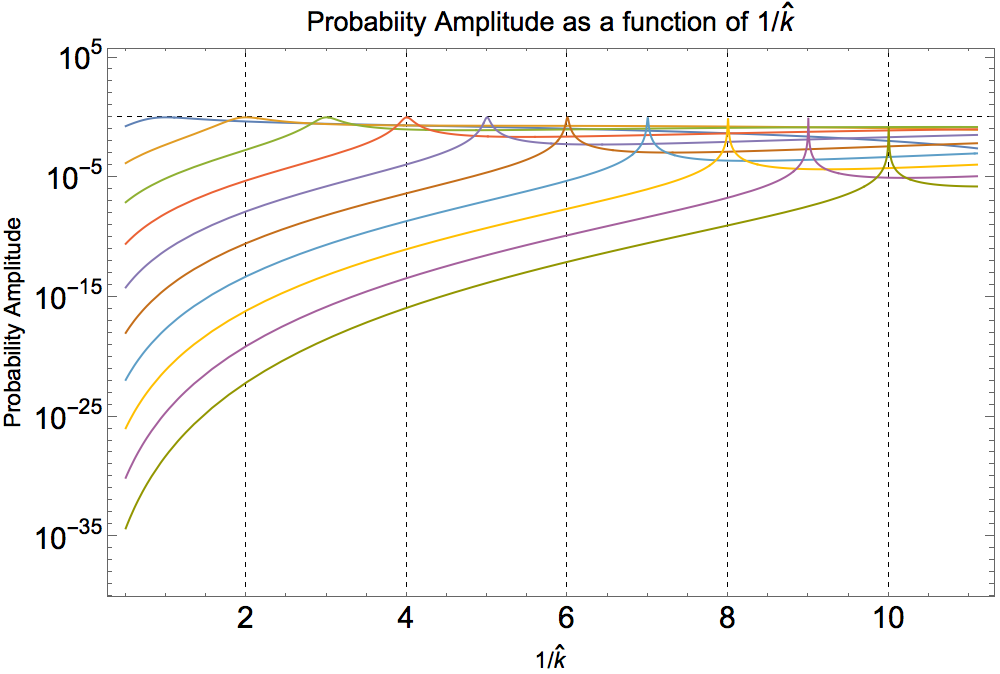
\includegraphics[width=0.95\textwidth]{assets/stimulated-single-frequency-resonances-k-orders.png}
\caption*{Resonances of different $n = 1/\hat k$.}
\end{figure}




\end{frame}


\begin{frame}{Single Frequency Matter Profile}

\begin{figure}
    \centering
    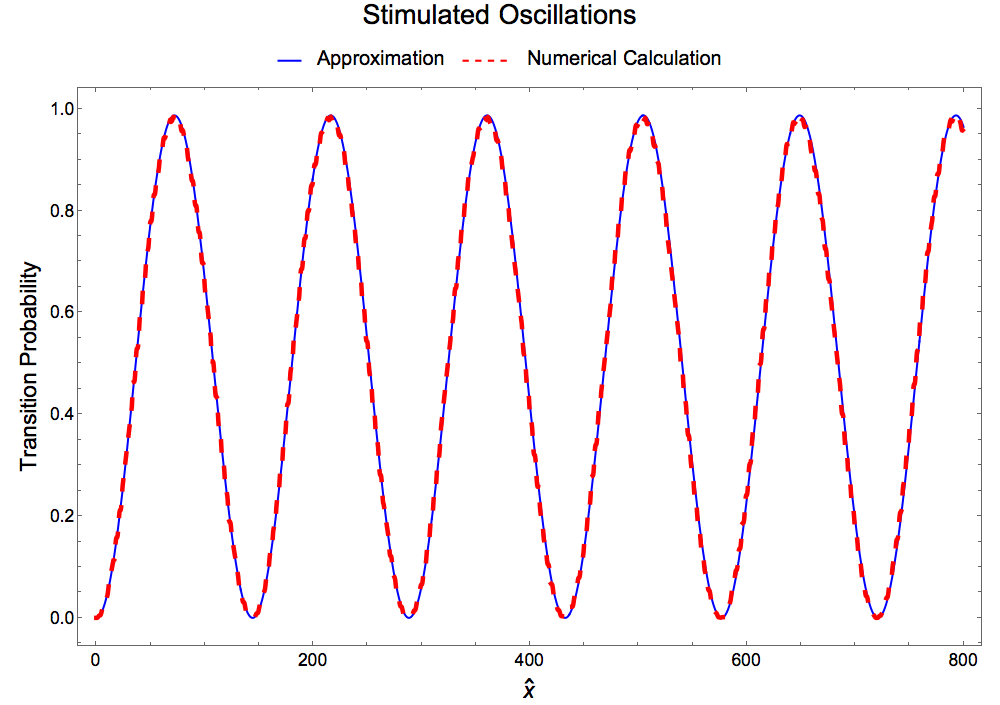
\includegraphics[width=0.9\textwidth]{assets/stimulated-oscillation-rwa-and-numerical.png}
    \caption*{$\hat A=0.1$, $\hat k=0.995$, $\theta_{\mathrm{m}}=\pi/6$}
\end{figure}

\end{frame}






% \subsection{Two-frequency Matter Profile}

\begin{frame}{Two-frequency Matter Profile}


\begin{figure}
    \centering
    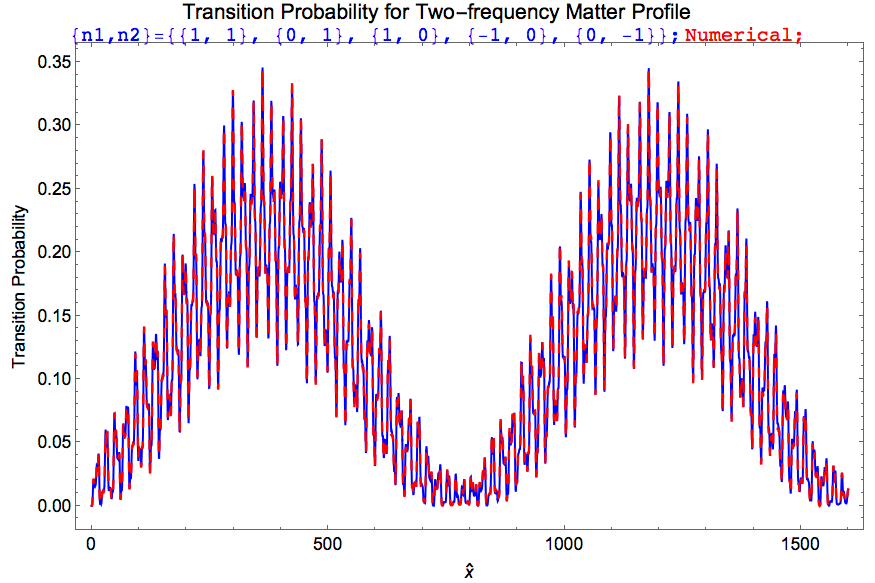
\includegraphics[width=\textwidth]{assets/2-freq-numerical-and-first-5-rwa.png}
    \caption*{$\lambda(x) = \lambda_0 + A_1\sin(k_1 x) + A_2\sin(k_2 x)$. $\hat k_1=0.3$, $\hat k_2=0.7$, $A_1=A_2=0.1$, $\theta_m=\pi/5$.}
\end{figure}


\end{frame}



%%%%%%%%%%%%%%%%%%%%%%%%%%%%%%%%%%%%%%%%%%%%%%%%%%%%%%%%%
%%%%%%%%% Dispersion Relation




\section{Neutrino Oscillations and Dispersion Relation}

\subsection{Neutrino Self-interactions}

\begin{frame}{Neutrino Self-interactions}

    
\end{frame}


\subsection{Linear Stability Analysis}

\begin{frame}{Linear Stability Analysis}

    
\end{frame}

\subsection{Dispersion Relation}

\begin{frame}{Dispersion Relation}
    
\end{frame}



%%%%%%%%%%%%%%%%%%%%%%%%%%%%%%
%%%% Neutrino Halo Problem



\section{Neutrino Halo Problem}



\begin{frame}{Neutrino Halo}

\end{frame}

\subsection{Flavor Isospin Picture}

\begin{frame}{Flavor Isospin}

\end{frame}


\subsection{Numerical Method}

\begin{frame}{Relaxation Scheme}


    
\end{frame}


\begin{frame}{Numerical Method}


    
\end{frame}




%%%%%%%%%%%%%%%%%%%%%%%%%%%%%%%%%%%%%%%%%%%%%%%%%%%%%%%
%%%%%%% Summary 


\section{Summary}

\begin{frame}{Summary}



\begin{itemize}\color{ao}
\item
The fact that neutrino flavor sates are not mass states causes vacuum oscillations.
\item
MSW resonance happens when matter potential cancels out the vacuum diagonal elements of the Hamiltonian.
\item
Even matter profile doesn't match MSW requirement, variation in matter profile can cause resonances.
\item
Single frequency perturbations in matter profile is a combination of many Rabi oscillations.
\end{itemize}



\begin{itemize}\color{red}
 \item
 How to understand and calculate systems with multi-frequency matter profile (turbulence).
 \item
 Combine periodic or even turbulent matter profile with neutrino self-interaction.
\end{itemize}




\end{frame}



\begin{frame}{Acknowledgement}

I am very thankful to my advisor Professor Huaiyu Duan, Dr. Sajad Abbar, and Dr. Shashank Shalgar, and Joshua Martin, for all the help in both research and life.

Supported by DOE EPSCoR grant \#DE-SC0008142 at UNM.

\end{frame}






    \begin{frame}[label=citations]{Citations}
      \framesubtitle{\TeX, \LaTeX, and Beamer}

      \justifying\TeX\ is a programming language for the typesetting
      of documents. It was created by Donald Erwin Knuth in the late
      1970s and it is documented in \emph{The \TeX
      book}~\cite{knuth84}.

      In the early 1980s, Leslie Lamport created the initial version
      of \LaTeX, a high-level language on top of \TeX, which is
      documented in \emph{\LaTeX : A Document Preparation
      System}~\cite{lamport94}. There exists a healthy ecosystem of
      packages that extend the base functionality of \LaTeX;
      \emph{The \LaTeX\ Companion}~\cite{MG94} acts as a guide
      through the ecosystem.

      In 2003, Till Tantau created the initial version of Beamer, a
      \LaTeX\ package for the creation of presentations. Beamer is
      documented in the \emph{User's Guide to the Beamer
      Class}~\cite{tantau04}.
    \end{frame}

    \begin{frame}[label=bibliography]{Bibliography}
      \framesubtitle{\TeX, \LaTeX, and Beamer}
      \begin{thebibliography}{9}
        \bibitem{knuth84}
            Donald~E.~Knuth.
            \emph{The \TeX book}.
            Addison-Wesley, 1984.
        \bibitem{lamport94}
            Leslie~Lamport.
            \emph{\LaTeX : A Document Preparation System}.
            Addison-Wesley, 1986.
        \bibitem{MG94}
            M.~Goossens, F.~Mittelbach, and A.~Samarin.
            \emph{The \LaTeX\ Companion}.
            Addison-Wesley, 1994.
        \bibitem{tantau04}
            Till~Tantau.
            \emph{User's Guide to the Beamer Class Version 3.01}.
            Available at \url{http://latex-beamer.sourceforge.net}.
        \bibitem{MS05}
            A.~Mertz and W.~Slough.
            Edited by B.~Beeton and K.~Berry.
            \emph{Beamer by example} In TUGboat,
              Vol. 26, No. 1., pp. 68-73.
      \end{thebibliography}
    \end{frame}

  \end{darkframes}



\end{document}
